%
% teil3.tex -- Beispiel-File für Teil 3
%
% (c) 2020 Prof Dr Andreas Müller, Hochschule Rapperswil
%
% !TEX root = ../../buch.tex
% !TEX encoding = UTF-8
%
\section{Anwendungen der Balkengleichung
\label{balken:section:teil3}}
Die Differentialrechnung ist von grundlegender Bedeutung für die Untersuchung und Lösung von Problemen im Zusammenhang mit der Balkengleichung. 
In diesem Abschnitt werden einige konkrete Anwendungen der Differentialrechnung in Bezug auf die Balkengleichung erläutert. 
Anschliessend werden Fallstudien und Beispiele vorgestellt, um diese Anwendungen weiter zu veranschaulichen.

\subsection{Praktische Anwendungen im Ingenieurwesen und Physik
\label{Praktische Anwendungen im Ingenieurwissenschaften und Physik}}
\begin{description}
\item[\textbf{Berechnung von Biegemomenten und Biegespannungen:}] Die Differentialrechnung wird verwendet, um das Biegemoment entlang eines Balkens zu bestimmen, der verschiedenen Belastungen ausgesetzt ist. 
Durch die Integration der Biegemomente entlang der Länge des Balkens kann die Biegelinie und somit die Krümmung des Balkens berechnet werden. 
Aus der Krümmung können dann die Biegespannungen mit Hilfe des Elastizitätsmoduls und des Trägheitsmoments ermittelt werden.

\item[\textbf{Optimierung von Balkenprofilen:}] Durch die Differentialrechnung können Ingenieure die optimale Geometrie von Balkenprofilen bestimmen, um bestimmte Anforderungen hinsichtlich Festigkeit, Steifigkeit und Gewicht zu erfüllen. 
Dies kann durch die Minimierung von Materialkosten oder das Maximieren der strukturellen Leistung erfolgen.

\item[\textbf{Analyse von statischen und dynamischen Verhalten:}] Die Differentialrechnung ermöglicht es, das statische und dynamische Verhalten von Balken unter verschiedenen Belastungen zu analysieren. 
Dies umfasst die Berechnung von Eigenfrequenzen, Schwingungsmoden und Schwingungsantworten, die für die Bewertung der strukturellen Stabilität und Leistung wichtig sind.

\item[\textbf{Entwurf von Tragstrukturen:}] Bei der Entwicklung von Tragstrukturen wie Brücken, Gebäuden oder Maschinenkomponenten ist die Differentialrechnung unerlässlich, um die strukturelle Integrität und Zuverlässigkeit zu gewährleisten. 
Sie ermöglicht es Ingenieuren, die Auswirkungen von Lasten und Belastungen auf die Struktur zu verstehen und entsprechende Designentscheidungen zu treffen.

\item[\textbf{Finite-Elemente-Analyse (FEA):}] Die Finite-Elemente-Methode, ein gängiges Werkzeug zur numerischen Lösung von Balkengleichungen, basiert auf der Differentialrechnung. 
Durch die Unterteilung des Balkens in kleine Elemente und die Anwendung von Differentialgleichungen auf jedes einzelne Element können Ingenieure komplexe strukturelle Probleme lösen und das Verhalten des Balkens unter verschiedenen Bedingungen simulieren. 
Für die Analyse beliebiger dreidimensionaler Strukturen wird die baustatische Methode allerdings deutlich schwieriger. 
Hier zeigt sich der Vorteil des Minimalprinzips: Die Variationsrechnung, insbesondere das Prinzip des kleinsten Energiepotentials. 
Die in der FEA verwendeten partiellen Differentialgleichungen sind die Euler-Ostrogradski-Differentialgleichungen des Minimumprinzips. 
Somit kann man mittels der FEA das Verhalten eines Balkens unter verschiedenster Bedingungen simulieren und komplexe Probleme lösen.

Eine interessante historische Anmerkung verdeutlicht die Bedeutung der Variationsrechnung in der Mechanik: Im 18. Jahrhundert versuchten Wissenschaftler, Gleichungen für Platten und Schalen mit der baustatischen Methode zu entwickeln, was jedoch zu falschen Ergebnissen führte. 
Erst durch den Einsatz der Variationsrechnung konnten die korrekten Gleichungen gefunden werden. 
Paul Funk beschreibt diese historische Entwicklung in seinem Buch über die Variationsrechnung. 
Die Balkengleichung ist dabei ein Sonderfall, bei dem sowohl die baustatische Methode als auch die Variationsrechnung erfolgreich angewendet werden können. 
\end{description}

\subsection{Fallstudien und Beispiele
\label{Fallstudien und Beispiele}}
Bei der Konstruktion von Brücken ist das Verständnis des Biegeverhaltens der Träger von entscheidender Bedeutung. 
Die Anwendung der Balkengleichung ermöglicht es Ingenieuren, präzise die Durchbiegung und auftretenden Biegespannungen entlang der Brückenbalken zu berechnen. 
Fallstudien untersuchen verschiedene Brückentypen wie Balkenbrücken, Bogenbrücken und Hängebrücken und zeigen auf, wie die Balkengleichung ihre strukturelle Integrität gewährleistet.

Ein herausragendes Beispiel für die Zuverlässigkeit von Tragwerken bietet die Reussbrücke Wassen, die 1972 im Rahmen der Gotthard Nordrampe erbaut wurde. 
\begin{figure} [h]
	\centering
	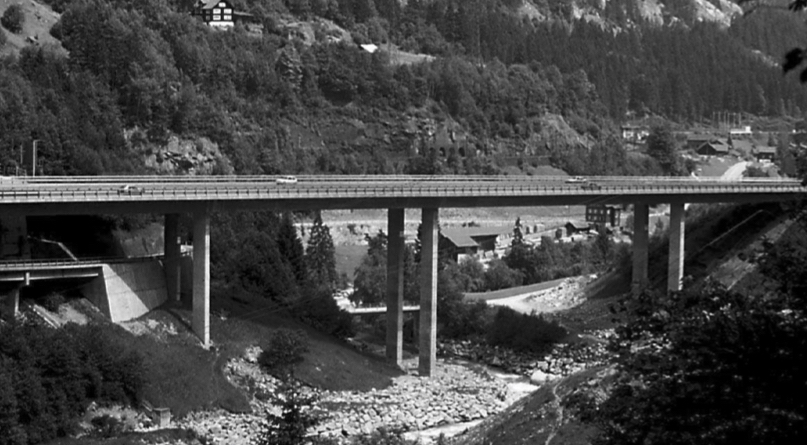
\includegraphics[width=\textwidth]{papers/balken/images/teil3/ReussbrueckeWassen1.jpg}
	\caption{Reussbrücke Wassen}
	\label{fig:Reussbrücke-Wassen}
\end{figure}
Im Jahr 2016 wurde die Brücke durch Hochwasser und Unwetter beschädigt, wobei das Fundament eines Pfeilers nahe dem Ufer der Reuss unterspült wurde. 
Trotz erheblicher Verformungen hielt die Brücke stand – ein eindrucksvolles Zeugnis für die Stabilität eines sorgfältig geplanten Tragwerks.
\begin{figure}
\begin{center}
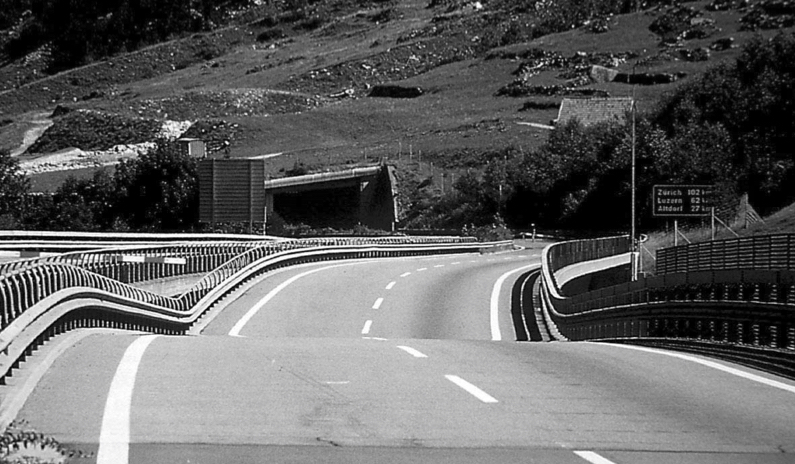
\includegraphics[width=\textwidth]{papers/balken/images/teil3/ReussbrueckeWassen2.jpg}
\end{center}
\caption{Verformungsvermögen}
\end{figure}
Die anschliessende Instandsetzung erforderte die Verstärkung des unterspülten Pfeilerfundaments sowie das Anheben des betroffenen Pfeilers in seine ursprüngliche Position mittels Pressen. 
Zusätzlich wurde eine Verstärkung im Brückenträger implementiert, um die strukturelle Integrität weiter zu verbessern. 
\begin{figure}
\begin{center}
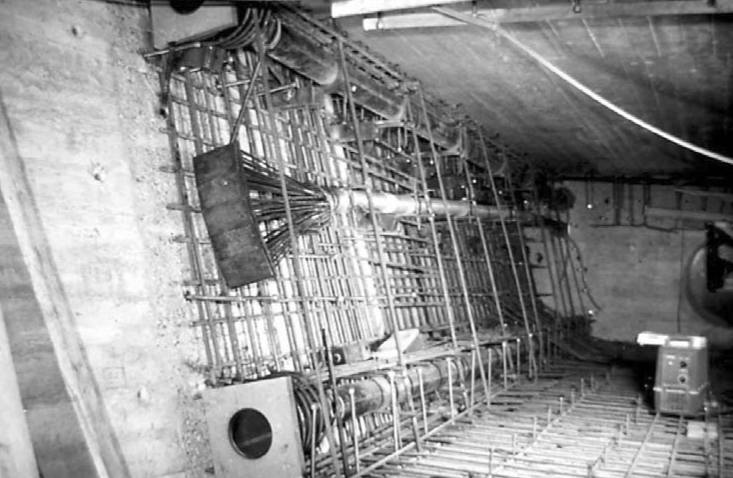
\includegraphics[width=\textwidth]{papers/balken/images/teil3/ReussbrueckeWassen3.jpg}
\end{center}
\caption{Verstärkung der Brückenträger}
\end{figure}
Trotz der Herausforderungen durch das Hochwasser und die Schäden kam es nicht zu einem katastrophalen Einsturz der Brücke, was die Wirksamkeit einer gründlichen strukturellen Planung und Instandhaltung verdeutlicht.

Neben Brücken finden Balken auch in Gebäuden Verwendung, beispielsweise für Tragwerke wie Decken, Dächer und Stützen.
Fallstudien in diesem Bereich befassen sich mit der Analyse des Biegeverhaltens von Gebäudeträgern unter verschiedenen Lastbedingungen. Ingenieure können mithilfe der Balkengleichung die erforderlichen Abmessungen von Stahlträgern berechnen, um die Lasten zu tragen, die durch das Gewicht des Gebäudes und der darin befindlichen Elemente entstehen.

Weitere bekannte Beispiele aus der Geschichte, die die Anwendung der Balkengleichung und deren Bedeutung für die Strukturintegrität illustrieren, sind:
\begin{enumerate}
\item Eiffelturm:
Die Anwendung der Balkengleichung ermöglichte es den Ingenieuren, die Trägerprofile und Verbindungen genau zu berechnen und den Eiffelturm zu einem der ikonischsten Bauwerke der Welt zu machen.
\item Brooklyn Bridge:
Bei der Konstruktion dieser Hängebrücke mussten die Ingenieure das Biegeverhalten der Tragseile, Hauptträger und Pfeiler genau verstehen, um die Lasten der Fahrbahn und des Verkehrs zu tragen.
\item Golden Gate Bridge:
Die Ingenieure analysierten sorgfältig das Biegeverhalten der Hauptträger und Pfeiler dieser Hängebrücke, die über die Bucht von San Francisco führt. Dies war erforderlich, um die enormen Lasten des Verkehrs und der Umwelt erfolgreich zu bewältigen.
\end{enumerate}
Diese praxisbezogenen Fallstudien und Beispiele verdeutlichen die zentrale Rolle der Balkengleichung bei der Planung und Konstruktion bedeutender Bauwerke wie Türmen, Brücken und anderen Tragstrukturen. 
Sie zeigen, wie Ingenieure die Prinzipien der Balkengleichung nutzen, um sicherzustellen, dass diese Strukturen den Belastungen standhalten und gleichzeitig sicher und zuverlässig bleiben.
Bei der Konstruktion von Brücken ist es von entscheidender Bedeutung, das Biegeverhalten der Träger zu verstehen. 
Die Anwendung der Balkengleichung ermöglicht es Ingenieuren, die Durchbiegung und die auftretenden Biegespannungen entlang der Brückenbalken präzise zu berechnen. Fallstudien untersuchen verschiedene Brückentypen, darunter Balkenbrücken, Bogenbrücken und Hängebrücken, und zeigen auf, wie die Balkengleichung eingesetzt wird, um ihre strukturelle Integrität zu gewährleisten.
